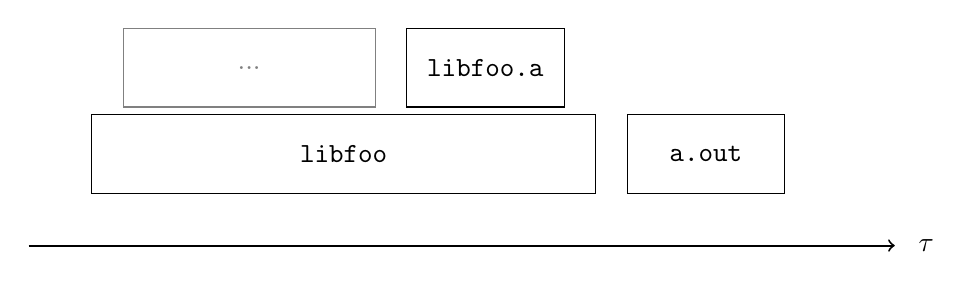
\begin{tikzpicture}
    \node[draw, minimum width=6.4cm, minimum height=1cm] at (4, 0) {\texttt{libfoo}};
    \node[draw, minimum width=2.0cm, minimum height=1cm] at (5.8, 1.1) {\texttt{libfoo.a}};
    \node[gray, draw, minimum width=3.2cm, minimum height=1cm] at (2.8, 1.1) {...};
    \node[draw, minimum width=2cm, minimum height=1cm] at (8.6, 0) {\texttt{a.out}};

%        \draw[dashed] (6.8, 1.6) -- (6.8, 3.0);
%        \draw[dashed] (7.2, 0.5) -- (7.2, 2.0);
%        \draw[dashed] (7.6, 0.5) -- (7.6, 1.0);

%        \node[font=\small, minimum width=6cm, text width=6cm] at (10, 3.0) {Завершение работы вложенной цели \texttt{libfoo.a}};
%        \node[font=\small, minimum width=6cm, text width=6cm] at (10.4, 2.0) {Завершение работы внешней цели \texttt{libfoo}};
%        \node[font=\small, minimum width=6cm, text width=6cm] at (10.8, 1.0) {Запуск целей, зависящих от \texttt{libfoo}};

    \node[font=\itshape] (time) at (11.4, -1.16) {$\tau$};
    \draw[line width=0.7pt, ->] (0, -1.16) to (11, -1.16);
\end{tikzpicture}